\chapter{Analisi}
\label{cap:analisi}
In questo capitolo analizzeremo il ragionamento che ci ha portato all'implementazione dei nostri esperimenti.

In particolar modo ci concentraremo sulle decisioni che sono state prese riguardo al representation language, che in Numsyth è contenuto nel file \textit{bias.pl}. Una volta che abbiamo deciso come vogliamo che il sistema ci spieghi il fatto su cui facciamo inferenza, cioè definito lo spazio di ricerca, diventa semplice definire la background knowledge (file \textit{bk.pl}) e le etichette degli esempi di training (file \textit{exs.pl}).

%%%%%%%%%%%%%%%%%%%%%%%%%%%%%%%%%%%%%%%%%
\section{Gestione delle tracce}
Un punto cruciale è stato definire come il sistema deve gestire gli stessi task in tracce diverse. Deve infatti essere consapevole che due task in tracce diverse che hanno lo stesso ID rappresentano la stessa implementazione con le stesse caratteristiche, ma non deve produrre una regola usando informazioni provenienti da tracce diverse.

Prendiamo come esempio la Figura~\ref{fig:trace_management}; questa è portata solo come esempio e ha poco senso in uno scenario reale, visto che le due tracce sono identiche. Quello che vogliamo è che il sistema non unisca le informazioni relative a quello che succede al \textit{Task1} nella prima traccia con quello che succede allo stesso task nella seconda traccia. È però importante che sappia che il \textit{Task1} è sempre lo stesso in entrambe le tracce, anche se non conosce le caratteristiche esplicite che il modello del sistema potrebbe fornirci.
\begin{wrapfigure}{L}{.5\textwidth}
    \centering
    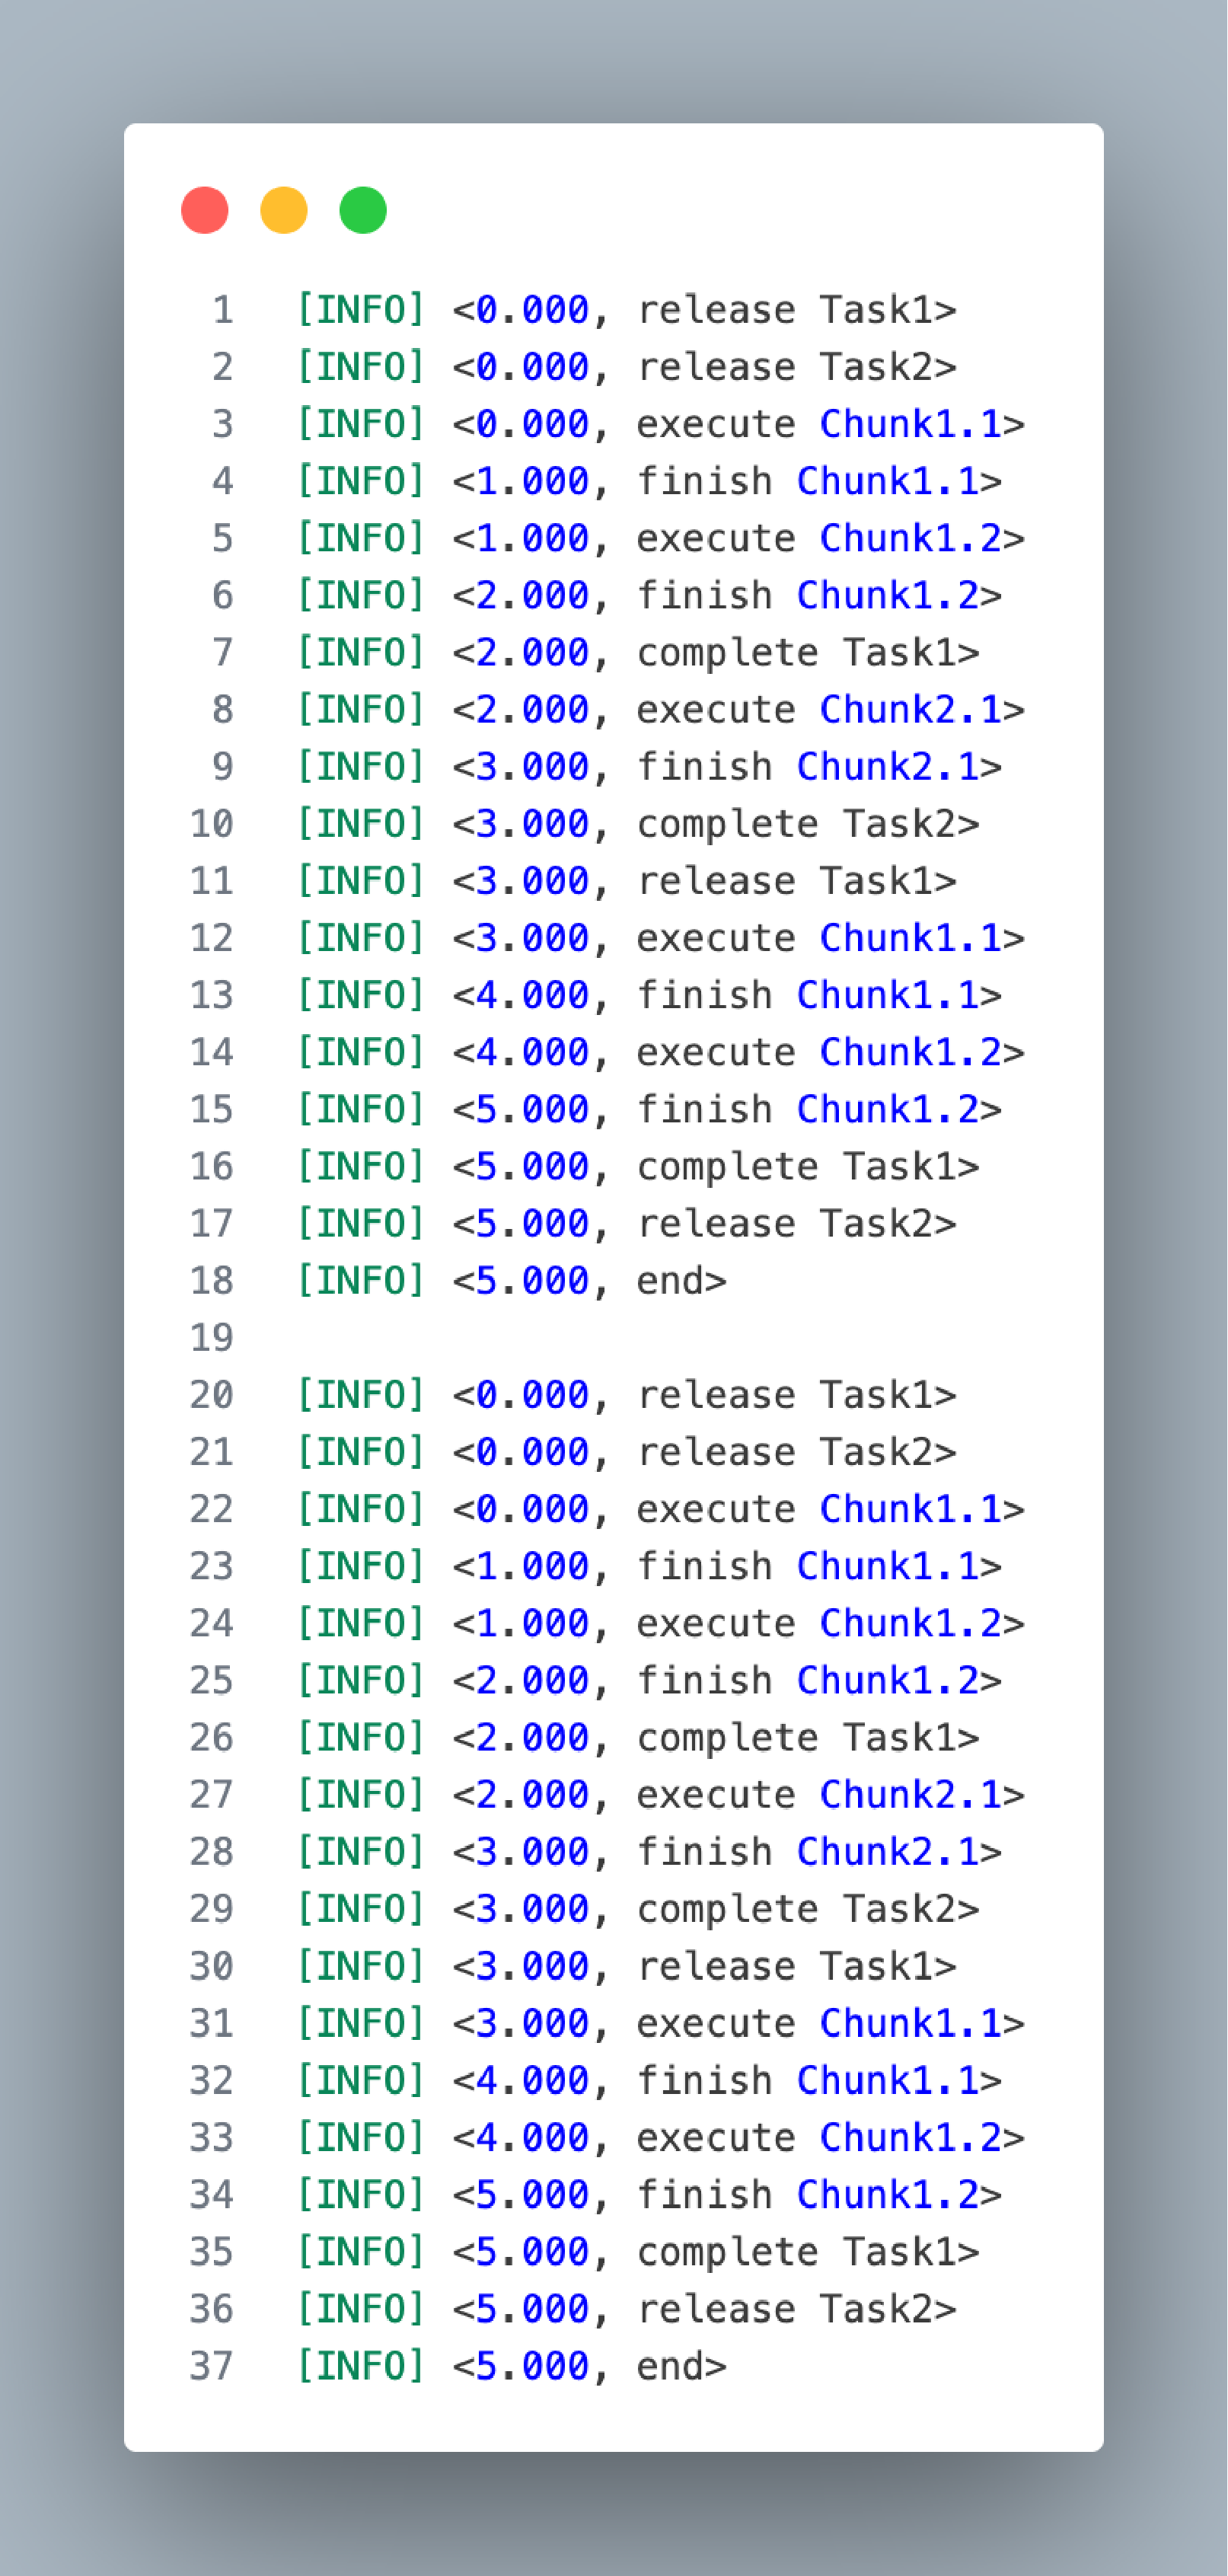
\includegraphics[width=.5\linewidth]{images/2-analisi/trace_management.pdf}
    \caption{\raggedright Trace management example.}
    \label{fig:trace_management}
\end{wrapfigure}

\myskip

A livello implementativo questo si traduce aumentando di un'unità l'arietà di ogni predicato, in modo da includere la traccia in cui l'evento è stato generato. Se ad esempio l'arietà di \textit{release} sarebbe 2, cioè se le sue variabili sono tempo e task, questa diventa 3, tempo, task e traccia.

%%%%%%%%%%%%%%%%%%%%%%%%%%%%%%%%%%%%%%%%%
\section{Gestione del tempo}
Un altro aspetto che ha richiesto attenzione è la gestione del tempo.

Siccome Numsynth gestisce valori numerici sia di tipo \textit{int} che \textit{float}~\cite{numsynth}, come prima idea potrebbe venire di utilizzare il tipo \textit{float} e prendere il tempo direttamente dal file di logging. Questo però comporterebbe avere una complessità maggiore e un tempo di training più lungo, vista la complessità nella gestione dei tipi in virgola mobile.

\myskip

Per semplificare l'addestramento è stato quindi deciso di rappresentare il tempo utilizzando \textit{int}. Siccome il sistema che genera le tracce mostra i tempi in millisecondi con tre cifre decimali, come si può vedere dalla Figura~\ref{fig:trace_management}, si è moltiplicato per $10^3$ il tempo mostrato. In questo modo è possibile usare tipi interi, ma si deve essere a conoscenza che il tempo va considerato appunto in microsecondi.

%%%%%%%%%%%%%%%%%%%%%%%%%%%%%%%%%%%%%%%%%
\section{Gestione dei task}
\label{sec:gestione-task}
Il nostro obiettivo è quello di fare inferenza su una traccia non vista non solo per predire il suo fallimento, ma anche per spiegarne il motivo, cioè per capire quale task è il responsabile di aver superato la sua deadline.

Con questa premessa diventa importante spiegare il fallimento di una traccia non solo sulla base degli eventi che definiscono la traccia, ma anche sulla base del comportamento dei task e dei chunk.

In questo modo non solo otteniamo una spiegazione sensata per i nostri requisiti, ma riduciamo anche la complessità del problema riducendo lo spazio di ricerca.

\myskip

A livello implementativo, quanto detto sopra si traduce definendo i predicati che esplicitano gli eventi in modo che contengano anche l'ID del task e del chunk che lo ha generato.

%%%%%%%%%%%%%%%%%%%%%%%%%%%%%%%%%%%%%%%%%
\section{Scelta predicati}
Negli esperimenti descritti nel Capitolo~\ref{cap:esperimenti} sono stati utilizzati diversi predicati. Questi, in un sistema di ILP, sono gli elementi base per costruire la regola.

I primi predicati usati sono quelli che compaiono nel file di log. Questi infatti li potremmo definire come predicati banali, in quanto se compaiono nel logging sicuramente sono di rilievo.

Un predicato non banale che è stato fondamentale negli esperimenti, e in particolare in quelli della Sezione~\ref{sec:execution_time}, è relativo al tempo di esecuzione dei vari chunk. Questo non compare direttamente nel file di log, ma tramite uno script che elabora l'inizio e la fine dell'esecuzione di un chunk è possibile ricavarlo.

Un predicato invece che non è stato considerato per la mancanza del modello è la differenza tra il completamento di un task e la sua deadline. Non essendo la deadline un'informazione inclusa nel log, per ricavarla servirebbe il modello del taskset, cosa che però non abbiamo. Per simulare questo valore potremmo usare la differenza tra il tempo in cui un task completa e il suo prossimo rilascio: questo ha senso solo se il task è puramente periodico, dove deadline relativa e periodo coincidono; se invece il task non è puramente periodico allora potrebbe avere un periodo molto lungo (e quindi essere rilasciato di rado) ma avere una deadline molto breve (e quindi richiedere un'esecuzione immediata).